\chapter{Observation and Data Reduction\label{sec:obs}}
We observed full single transit of each of our target with the OAO/MuSCAT (see $\S$\ref{sec:muscat} for technical details) between 2016/08  and 2017/04. The image position was selected such that the target and many comparison stars were imaged together within the FOV. %among which we chose GSC 03465-00123 (V= 13.2).
%Due to the uncertain ephemeris, propagated error since last observation 3 years ago 
Whenever possible, we started the observation at least $\sim$1 hour before/after the ingress/egress to cover the full transit and obtian long baseline. The sky was perfectly clear with no moon visible during the observations. %The condition was photometric through the observations. 
The g-,r-, and z-bands images were taken with exposure times adjusted such that all stars have value counts within linearity regime of the detector, yielding different number of raw frames for each band. The typical size of the PSF was $\sim$ 11 pixels ($\sim$4") in radius.
%The exposure time was set to XX s and the dead time (including the CCD readout time of XX s and other setup times) was about XX s (duty cycle of XX\%). 
The telescope auto-guider managed to keep the centroid on the three detectors with %standard deviation 
median value of less than 2 pixels in both X and Y directions. The observation details are summarized in Table~\ref{tab:obs}.

\section{Standard Reduction}
%%%basic reduction: dark, flat, bias, linearity correction 
Primary data reduction, including bias subtraction and flat fielding, and aperture photometry was carried out with a customized pipeline by \cite{Fukui2011}. 
%The raw images were dark-subtracted and flat-fielded in a standard manner. 
To create the flat field, we median combined 50 dome flat images for each band that were obtained on the observing night. Note that we convert the time stamps, which is recorded in the FITS headers in units of Modified Julian Day (MJD) based on Coordinated Universal Time (UTC), to Barycentric Julian Day (BJD) based on Barycentric Dynamical Time (TDB) i.e. BJD$_{\rm{TDB}}$ system using the algorithm by \cite{Eastman2010}. 
%Corrections to the barycentre are more precise than the heliocentre, because the barycenter is a fixed point where gravity is constant. For maximum accuracy you want to have your barycentric corrected times in a timescale that has always ticked at a uniform rate, and ideally one whose tick rate is related to the rate that a clock would tick at the barycentre. For this reason, barycentric corrected times normally use the TDB timescale:
%http://astroutils.astronomy.ohio-state.edu/time/

\begin{table}
\centering
\caption{Observation log of each of our targets and results of aperture photometry.}
\label{tab:obs}
\begin{tabular}{lllll} \hline
                                       &HAT-P-44      &HAT-P-12        &WASP-21       \\ \hline
Observation calendar (UT)    & 2017/02/15  & 2017/04/29  & 2016/08/12\\
%comparison stars & & & & \\
exposure times (s) &60,30,60 & 40,20,50 & 50,20,50 \\
no. of data images & 376,703,376 & 349,623,277 & 483,1072,465 \\
$\sigma_{dx}$ (pix)& 0.95, 0.40, 0.64& 0.57, 0.37, 0.30 & 0.97, 0.77, 0.71 \\
$\sigma_{dy}$ (pix)& 0.50, 0.35, 0.51& 0.81, 0.39, 0.31 & 1.21, 0.62, 0.45 \\ \hline
aperture radius (pix) & 11 & 18 & 11 \\
no. of data points & 376,703,374 & 349,623,277 & 483,1072,465 \\
\hline
\end{tabular}
\end{table}

%n high-speed (2 MHz) readout mode, while the  band images were taken with the exposure time of 30 s in low-seed (100 kHz)readout mode\footnote{The reason for using the low-speed readout mode was that the CCD camera for $z_{s,2}$ band produced uncorrectable systematic noises only in the high-speed readout mode. The camera was repaired after the observation, and the problem has been fixed.}, resulting in the observing cadences of 14 s, 14 s, and 43 s for the $g'_2$- and $r'_2$ and $z_{s,2}$ band, respectively. 

\section{Aperture Photometry}\label{sec:apphot}
After the raw images were processed by performing standard over-scan correction, de-biasing, and flat-fielding (see $\S$\ref{sec:obs}), we perform aperture photometry using a customized code detailed in \cite{Fukui2011}. This custom pipeline also calculates the photometric error, including photon noise, detector noise, and scintillation noise, used as initial estimate of uncertainties in transit modeling. We summarize the steps in aperture photometry as follows.

First, we create several trial light curves using different aperture sizes and combinations of comparison stars for each observation. For the comparison stars, we select such stars that are neither saturated, nor variable. 
The aperture radius was chosen to give the smallest scatter in the flux outside of the transits, and was generally \textbf{9 to 15} pixels. %\textbf{
The reference flux was obtained by summing the flux of the comparison stars. The flux of the target star was then divided by this reference signal to produce a time series of relative flux. Each time series was normalized to have unit flux outside of the transit. After excluding obvious outliers (>50-sigma from the median), the number of data points used in the analysis in each data set is summarized in Table~\ref{tab:obs}.
%We then check the all trial light curves by eye and eliminate obviously poor-quality ones.

%%%aperture optimization
Second, in order to select the most appropriate light curve for each observation and its baseline correction model for OOT phase, we adopt the BIC for our analyses. We fit the trial light curves with an analytic transit light curve model and various baseline models simultaneously (see $\S$ \ref{sec:sysmodel}). 

%To determine the optimal apertures to use in our analysis, we generate and inspect the $\beta$ and $\sigma$ diagnostics. %plotted in Fig.~\ref{fig:}. 
%We find that the minimum red noise aperture (\textbf{XX} pixel) is frequently consistent with the minimum white noise aperture to within a few tenths of a pixel (\textbf{XX} pixel).

\section{Light Curve Modeling: Bayesian Framework}
%intro to bayesian inference
%http://iopscience.iop.org/article/10.1086/500802/pdf
A transit light curve is basically composed of two components: transit and systematics. We follow Bayesian framework (e.g. \cite{Parviainen2017}; \cite{Diaz2017}) in modeling both transit and systematics simultaneously in three MuSCAT bands for each data set. %The goal is to estimate the posterior probability distribution (as opposed to a single point estimate) of the model parameters using the Bayes' Theorem.
In Bayesian modeling, we do not get a single estimate for our model parameters as we would with maximum likelihood estimation. Instead, we get a complete posterior distribution for each model parameter, which quantifies how likely different values are for that model parameter. For example, with few data points our estimation uncertainty will be high reflected by a wide posterior distribution. As we gather more data, our uncertainty about the model parameters will decrease and we will get an increasingly narrower posterior distribution. There are many more benefits to the Bayesian approach, such as the ability to incorporate prior knowledge.

\paragraph{Bayes' Theorem}
The posterior probability density given a parameter vector $\theta$ and observational data $D$ is described by the Bayes' theorem as
\begin{align}
P(\theta|D)&=\frac{\Pi(\theta) \times \mathcal{L}(D|\theta)}{M(D)} \\
& \propto \Pi(\theta) \times \mathcal{L}(D|\theta)
%\rm{Posterior \propto Prior \times Likelihood}
\end{align}
where $\Pi(\theta)$ is the prior probability of $\theta$, $\mathcal{L}(D|\theta)$ is the likelihood of the data given $\theta$, and $M(D|M)$ is a normalizing factor also called the marginal. Since we use Markov Chain Monte Carlo algorithm to sample the posterior distribution (see $\S$ \ref{sec:MCMC}), the marginal can be ignored and so the Bayes' theorem can be simplified as given above.

\paragraph{Model Likelihood}% of Transit \& Systematics Model}
Assuming that the parameters in our model are independent, identically distributed (iid) random variables, we can expect that the residual follows a Gaussian distribution:
\begin{equation}
\label{eq:likelihood}
\mathcal{L}(D|\theta) = N(\mu,\sigma) = \frac{1}{\sqrt{2\pi \sigma^2}} \exp \Big(-\frac{(x-\mu)^2}{2\sigma^2} \Big)
\end{equation}
where $N(\mu,\sigma)$ is the normal distribution with mean model $\mu$ and standard deviation $\sigma$. Here $\mu$ is the transit model, $x$ is data divided by the systematics model, and $\sigma$ is the measured photometric uncertainty.

The likelihood is a product of individual observation probabilities, and has the unfortunate tendency to end up being either very small or very big. To avoid computational overhead, it is better to work with log probabilities instead, so that
\begin{align}
\ln \mathcal{L}(D|\theta)& = \ln\Big[(2\pi\sigma^2)^{-\frac{1}{2}}\Big] +\ln \Big[\exp\Big(-\frac{(x-\mu)^2}{2\sigma^2}\Big)\Big] \\
& = -\frac{1}{2}\ln(2\pi) -\frac{1}{2}\ln \sigma^2 -\frac{(x-\mu)^2}{2\sigma^2} \\
&= -\frac{1}{2}\Big[\ln(2\pi) +2\ln\sigma +\Big(\frac{x-\mu}{\sigma}\Big)^2\Big]
\label{eq:loglikelihood}
\end{align}
%where we can drop constant terms since the MCMC samplers only require something proportional to $\ln{P(\theta)}$. 

\subsection{Transit Modeling}\label{sec:transitmodel}
We begin by modeling the light curves in flux scale using a combination of in-transit and out-of-transit (OOT) models, described by
\begin{equation}\label{eq:lc}
F_{rel}=F_{out}\times F_{in} \\
\end{equation}
where $F_{rel}$ is the relative flux (raw flux of target star divided by flux of comparison star obtained from relative photometry), $F_{in}$ is the in-transit model, and $F_{out}$ is the OOT model including the systematics.
%We fit the light curve with the analytic model of the form $F_{\rm{white}}(t) = S_{\rm{white}}(t)\times T_{\rm{white}}(t)$, where $S_{\rm{white}}$ is a systematics model and $T_{\rm{white}}$ is a transit model in flux scale.

There are several analytic transit models but the $de$-$facto$ standard are the ones by \cite{MandelAgol2002} and \cite{Gimenez2006}. We adapt the former for this study. The transit parameters in the Mandel-Agol model are:
\begin{itemize}[noitemsep]
% \item $t$:\; time \\
 \item $R_p/R_s$: planet-star radius ratio ($R_p/R_s^2\equiv$ transit depth)\\
 \item $u$: limb-darkening coefficients\\
 \item $t_c$:    transit center\\
 \item $P$:     orbital period\\
 \item $a_s$:   a/Rs: scaled semi-major axis\\
 \item $i$:     inclination\\
 \item $e$:     eccentricity\\
 \item $\omega$:     argument of periastron\\
\end{itemize}
The Mandel-Agol model was evaluated using the \verb'PyTransit'\footnote{https://github.com/hpparvi/PyTransit} light curve modeling tool implemented in Python (\cite{Parviainen2015}), which requires at least the first 6 transit parameters above. We adapt the published values including their uncertainties summarized in Table~\ref{tab:init}. On the following, we define relations used to set the priors on relevant parameters.

\paragraph{Priors for Transit Parameters}
In our MCMC analysis ($\S$ \ref{sec:MCMC}), the free parameters are allowed to vary over the range of plausible values set by the prior. 

\begin{itemize} %enumerate
\item inclination, $i$, and impact parameter, $b$:\\
Following the prescription by \cite{Parviainen2017} for modeling the transit light curves, we used $b$ instead of $i$ as a free parameter, and assumed $\omega=90$ and $e=0$, as found (or assumed) in previous publications. 
%e.g. HAT-P-12: Hartmann+2009; Sada & Ramon-Fox 2016
%HAT-P-12b:
%Hartman et al. (2009) derive an orbit with zero eccentricity from the radial velocity data presented in the discovery paper. Recently, Knutson et al. (2014) include a few more radial velocity measurements, but they also calculate an eccentricity for the orbit that is consistent with zero. Thus, we also adopt a circular orbit for this system in our modeling. 
%WASP-21b
%Bouchy et al. (2010) found that including a small non-zero eccentricity to the fit does not improve the results. Hence, they concluded that the eccentricity is consistent with zero.
%This also has advantage of for simplicity and more efficient sampling. ($\S$\ref{sec:MCMC}). 
\begin{align}
b &= a_s\cos\Big(\frac{1-e^2}{1+e\sin\omega} \Big) \; \in \; [0,1+k] \\ 
i  &= \arccos\Big( \frac{b}{a_s} \Big[ \frac{1+e\sin \omega}{1-e^2} \Big ] \Big)
\end{align}

\item semi-major axis, $a$, \& stellar density, $\rho_s$:\\
We used the relation between scaled semi-major axis and stellar density defined in \cite{SeagerMallen-Ornelas2003}:
\begin{align}
a_s &= \Big( \frac{G\rho_sp^2}{3\pi}\Big)\\
\rho_s &= \frac{3\pi a^3_s}{Gp^2}  \label{eq:rho_star}
\end{align}
%\item eccentricity, $e$, and argument of periastron, $\omega$:\\
%See Ford (2005); Anderson et al. (2011)
%\begin{eqnarray}
%x = \sqrt{e}\cos \omega, y = \sqrt{e}\sin \omega \\
%e = x^2+y^2, \omega = \arctan(y/x)
%\end{eqnarray}

\item Stellar limb darkening in transit modeling\\
Limb darkening is an optical effect where the center part of the disk appears brighter than the edge or limb of the image. Depending on the model, limb-darkening can be parameterized by $n$ coefficients (hereafter called LDC). A common approach is to use the quadratic ($n$=2) limb-darkening law %which was first proposed by Kopal (1950). We adopt the quadratic limb-darkening law because it is simple and intuitive, flexible to explore a range of profiles plus a fairly compact, efficient structure \cite{Kipping2013}). 
described by:
\begin{equation}
\frac{I(\mu)}{I(1)} = 1 − u_1(1 − \mu) − u_2(1 − \mu)^2
\end{equation}
where $I(\mu)$ is the specific intensity of a star, $\mu=\cos \theta$ is the cosine of the angle between the line of sight and the emergent intensity, and $u_1, u_2$ are the LDCs.

%The LDCs are mutually correlated and degenerate with the planet-star radius ratio Rp/Rs and impact parameter. Fixing LDCs leads to biased parameter estimates (Csizmadia et al. 2013; Espinoza \& Jordan; see also Muller et al. 2013 for counter-argument). Allowing the LDCs to be free parameters enables propagation of uncertainties in the stellar parameters to properly account for uncertainties in the final planet parameters. 

Fixing the limb darkening coefficients has been shown to bias measurements of the transit depth (\cite{Espinoza2015}). Yet, when left as free parameters, these coefficients are strongly correlated in MCMC retrievals (Pal 2008; Kipping 2013). 
%To reduce a correlation between the quadratic limb-darkening coefficients u1 and u2, and to appropriately estimate uncertainties for other parameters, 
We solve this problem by using the triangular sampling method of \cite{Kipping2013}. This re-parameterization from $u$- to $q$-space involves making a rotation to new principal axes:
\begin{align}
q_1 &= (u_1+u_2)^2\\
q_2 &= \frac{u_1}{2(u_1+u_2)} \; \in \; [0,1] \\
u_1& = 2\sqrt{q_1}q_2 \\
u_2& = \sqrt{q_1}(1-2q_2)
\end{align}
%In our modeling, we adapt LDC in ($q_1,q_2$)-space constrained by model-based informative priors (e.g. Claret 2013).

This transformation %(see also Fig.~\ref{fig:q_to_u}) 
allows us to efficiently obtain only physically allowed limb-darkening coefficients. We used normal priors for $q_1 \& q_2$ with center and width defined by the theoretical values for limb-darkening coefficients %using PHOENIX-calculated stellar limb darkening profiles
(\cite{Claret2012}). 
%We refer the tables of quadratic limb-darkening parameters by Claret et al. (2013) and compute allowed w1 and w2 values for the stellar parameters presented in Table 1.
%We determine Gaussian limb darkening priors using open source Python package \verb'LDTk'\footnote{https://github.com/hpparvi/ldtk} (\cite{Parviainen2015}), which relies on the PHEONIX stellar model grid of \cite{Husser2013}. In brief, the uncertainties of stellar paramters are propagated into the limb darkening coefficients using a library of stellar atmosphere models in conjunction with the transmission function of the MuSCAT bandpass.
Given the Table available online\footnote{http://adsabs.harvard.edu/abs/2012yCat..35460014C}, we interpolated the theoretical limb-darkening coefficients using the limbdark package\footnote{https://github.com/john-livingston/limbdark} assuming the stellar parameters as shown in Table \ref{tab:ldc} where the uncertainties define the resulting LDC prior widths. %The priors for the MCMC analysis are summarized in Table~\ref{tab:prior}
%A normal prior is also used for stellar density computed using the equation prescribed by Seager et al. (2000). 
We used uniform priors for the remaining transit parameters such as the impact parameter, $b$, from which inclination was computed. 

\begin{table}
\centering
\caption{Stellar parameters used for computing the prior values for quadratic limb-darkening coefficients.}
\label{tab:ldc}
\begin{tabular}{lllll} \hline
          &HAT-P-44      &HAT-P-12        &WASP-21     \\ \hline
$T_{\rm
{eff}}$   &5300$\pm$100  &4650$\pm$60     &5800.0$\pm$100.0 \\%&6100$\pm$65    \\
log g     &4.460$\pm$0.06&4.2$\pm$0.1      &4.190$\pm$0.03  \\%&4.610$\pm$0.01  \\
Fe/H      &0.33$\pm$0.1  &-0.290$\pm$0.05 &-0.46$\pm$0.11   \\ \hline %&-0.200$\pm$0.06\\ \hline
\end{tabular}
\end{table}
\end{itemize}

\begin{table}
\centering
\caption{Initial values for the transit parameters used in evaluating Mandel-Agol model.}\label{tab:init}
\begin{tabular}{lllll} \hline
          &HAT-P-44b      &HAT-P-12b        &WASP-21b   \\ \hline
$P$  (d)         & 4.301219 &3.2130598 &  4.322482\\
$(R_p/R_s)^2$  & 0.01804 & 0.01977 & 0.01082 \\
$b$                 & 0.172 &  0.211 & 0.23 \\
%$t_c$ (d)         & 7.8e3+0.22-2450000 & 2.457873e6+0.23 &  2.457613e6+0.19 &\\
$t_c$ (d)         & 2442199.78 & 2457873.23 &  2457613.19\\
$a_s $                & 11.52 & 11.80 & 11.52 \\
$i$ (deg)          & 89.10 & 89.00 & 88.75 \\ 
\hline
\end{tabular}
\end{table}
%priors
%t14 = 0.13020
%_t14 = 0.09740
%_t14 = 0.1398

\begin{comment}
An alternative approach to solve %the bias of transit depth and 
correlation in MCMC retrieval by Rackham et al. (2016) in which $q_1$ is defined as a free parameter and $q_2$ is fixed to values obtained from a PHOENIX atmospheric model (Husser et al. 2013). However, we found that this is not necessary as our results confirm that there is no correlations among all limb darkening coefficients in all passbands after inspecting their joint posterior distributions as shown in Fig~\ref{fig:q1q2}).
%NOTE: Instead of constraining the limb darkening model coefficients, Parviainen (2013) constrained the shape of the stellar limb darkening profile by fitting a stellar limb darkening profile created using specific intensity spectra library by Husser et al. (2013); the profile-based approach reduces the problems encountered with the limb darkening coefficient correlation. 
\begin{figure*}
	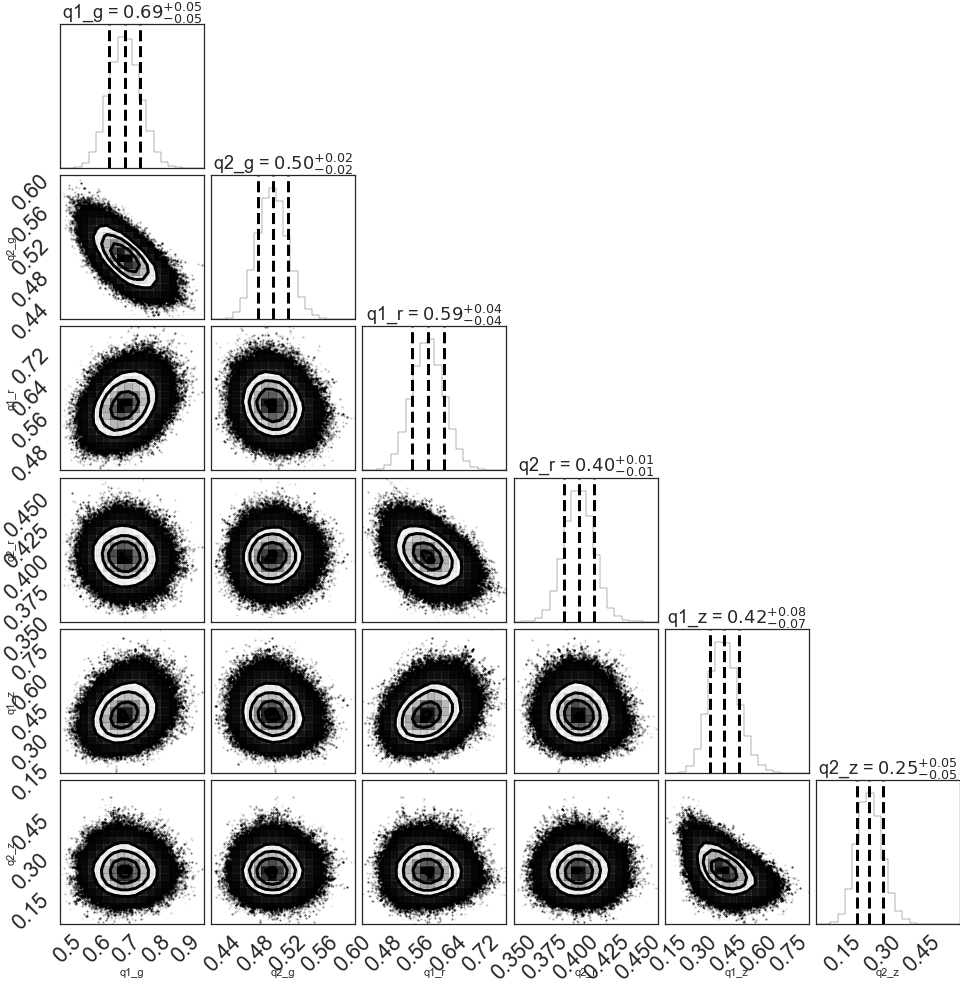
\includegraphics[width=1.5\columnwidth]{figures/limbdark_q1q2.png}
    \caption{Corner plots of limb-darkening coefficients $q_1$ and $q_2$ for each g-,r- and z-band. The joint posterior distributions show no correlation among the coefficients.
    }
    \label{fig:q1q2}
\end{figure*}
\end{comment}

\subsection{Systematics Modeling}\label{sec:sysmodel}
%See Luger+2017 notes
A transit light curve contains various information. Aside from the transit signal, it also (generally) contains systematic noise and photometric noise, as shown in Fig.~\ref{fig:noise_sources}. Here, we refer systematics as a catch-all term that accounts for the noise in the light curve except photometric noise. Systematics is largely composed of (but not limited to (1) stellar variability, (2) instrumental noise (e.g. read noise, tracking problems), (3) telluric/atmospheric variability, some of which manifest in out-of-transit (OOT) phase of each dataset. Systematics in the OOT phase is more pronounced in HAT-P-12b (Fig.~\ref{fig:hatp12_opt}) and HAT-P-21b (Fig.~\ref{fig:wasp21_opt}) raw light curves especially towards end of the observation.
%slow variability in the brightness of GJ1214 itself or comparison stars, changing airmass, position changes of the stars on the detectors, or high sky background, and so on. 
\begin{figure}
\centering
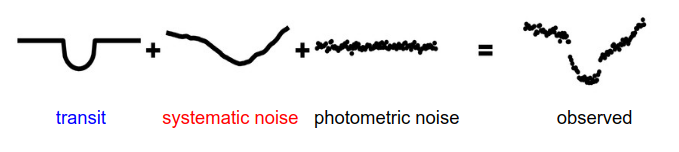
\includegraphics[width=15cm]{figures/noise.png}
\caption{General components of a transit light curve including noise.}
\label{fig:noise_sources}
\end{figure}
%What we would like to do is to model all of them together and at the same time (i.e simultaneous) to get the best fit parameters; not model them separately by removing systematic first and then fitting for transit parameters (or vice-versa).
Because the difference in the expected transit depths at a given passband can be smaller relative to the amplitude of the systematic noise, imperfect systematic correction can easily cause biases in the transit parameters. Hence, systematics should be accounted for correctly to ensure unbiased results.%high photometric accuracy.

As in \cite{Fukui2016a} (see also \cite{Luger2017}), we adapted the usual parameterization of $F_{out}$ as a linear combination of  constant coefficients (or weights), $w$, and observables, $X$,
\begin{equation}
F_{out}= \Big(w_0+\sum w_iX_i \Big) \times F_{in}
%F_{out}=k_0 \times 10^{=0.4 \Delta m_cor}= \sum k_iX_i
\end{equation}
where $X$ contains auxiliary information obtained during the observation such as  target's FWHM, change in stellar position on the detector, airmass, etc. 
%Using Maximum Likelihood Estimation (MLE) to compute/optimize $w$ is not recommended (and will most likely fail) because we don't have good guesses for the initial values of the constant coefficients. Remember in our transit modeling, we have good guesses for limb-darkening coefficients, transit center, etc.

% $w$ is a nuisance parameter\footnote{A nuisance parameter is one that is required in order to model the process that generates the data, but is otherwise of little interest.}
Computing the coefficients $w_i$ is simply doing multiple regression:
$$
y_i=10^{-0.4S}
$$
where 
\begin{equation}
S=w_0+\sum_{i=0}w_iX_i,
\end{equation}
given two or more variables in $X$. In vector form, $y= X \cdot w$ where $w$ can be solved with linear algebra,
\begin{align}
X^T \cdot y& = X^T \cdot X \cdot w \\
w&=(X^T \cdot X)^{-1} \cdot X^T \cdot y 
\end{align}
Here $y$ is the function we want to model (e.g. OOT flux normalized by the transit model) and $X$ can be composed of any auxiliary observables that can reasonably explain the variability, including airmass, centroid position of target in the detector, etc. Since our raw light curves show apparent trend in OOT phase, we included the baseline (i.e. $w_0+w_1t$) as default in the systematic model of each data set. 

There is no rule on how to determine the best or correct set of auxiliary observable to put in $X$. It is reasonable however to use those vectors that are correlated with the function that we want to model. Thus, we first consider observables that are correlated with the OOT phase. A sample pairplot for HAT-P-44b observables is shown in Fig.~\ref{fig:pairplot} which visualizes the correlation among variables. 
\begin{figure}
\centering
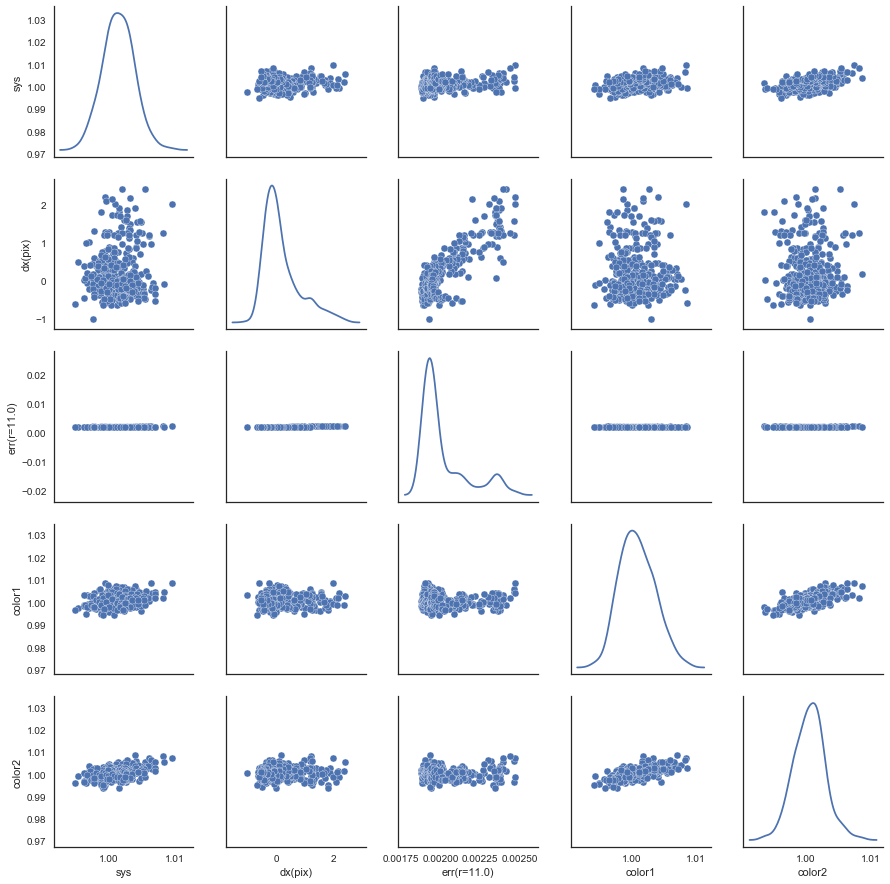
\includegraphics[width=12cm]{figures/best_observables.png}
\caption{An example pair plot of OOT flux and observables showing no apparent correlations (in the off-diagonal) %and density (along diagonal) 
among variables in g-band of HAT-P-44b data set.}
\label{fig:pairplot}
\end{figure}

Intuitively, the more parameters used in the model, the better the fit. 
%When fitting models, it is possible to increase the likelihood by adding parameters, but doing so may result in overfitting. The BIC resolves this problem by introducing a penalty term for the number of parameters in the model.
When selecting a good model however, it should have a balance between goodness of fit and model simplicity. Thus, we use Bayesian Information Criterion (BIC; \cite{Schwarz1978}) to objectively determine which observables to include in the model. BIC is defined as
\begin{equation}
BIC = \chi^2 +d\log N
\end{equation}
where $\chi^2$ is the standard chi-square, $N$ is the number of data points in the light curve and $d$ is the number of dimensions or parameters in the model. Between two competing models, the one with smaller BIC value is preferred. The observables used in each data set and their BIC values are summarized in Table~\ref{tab:bic}. %The adapted observables are shown in bold.
Although a simple 2-parameter baseline model yields lowest BIC value, we adapted a 5-parameter model because it models the variability better especially in the OOT phase. %A separate method for model selection using the Bayesian evidence is discussed in $\S$\ref{sec:model_selection}. The BIC is determined solely from the highest likelihood value, making it easier to calculate than K. Models with lower BIC values are generally favored. Note, however, that the BIC is a less accurate method for distinguishing between models than is K.

\begin{table}
\centering
\caption{BIC values for a representative sample of combinations of observation.}
\label{tab:bic}
\begin{tabular}{lllllllllllll}
model  & \multicolumn{4}{l}{HAT-P-44b}          & \multicolumn{4}{l}{HAT-P-12b}          & \multicolumn{4}{l}{WASP-21b}           \\ \hline
       & BIC & rms & $\beta$ & BIC & rms & $\beta$ & rms$\times\beta$ & BIC & rms & $\beta$ \\
g-band & \multicolumn{12}{l}{}                                                                                                    \\
$k_z$  & 1262.88    & 0.0018    & 1.1515       &   0.002   & 3766    & 0.0019    & 2.5096        &  2825   & 0.0008     & 3.3068                   \\ \hline
r-band & \multicolumn{12}{l}{}                                                                                                    \\
$k_z$  & 2365.70    & 0.0017    & 1.3033       &  0.002    & 6260    & 0.0019    & 2.2240        & 9345    & 0.0011    &  2.6869                   \\ \hline
z-band & \multicolumn{12}{l}{}                                                                                                    \\
       &     &     &         &                 &     &     &         &                  &     &     &         &    \\
$k_z$  & 1211.68    & 0.0020    & 1.3345       &   0.002   & 3010    & 0.0019  &  1.8684       & 4030    &  0.0011   & 2.9127                     \\ \hline
\end{tabular}
\end{table}
                              
\begin{comment}
Fukui et al. (2016) introduced a parameterization of baseline systematics which takes account of the second-order extinction effect. The applied function is:
$$
m_t(t) = M_{tr} + w_0 + w_tt + w_cm_c(t) + \sum w_iX_i
$$
where $m_t$ and $m_c$ are the apparent magnitudes of the target star and comparison stars, respectively, $M_{tr}$ is a transit model in magnitude scale, $t$ is time, $X_i$ is auxiliary observables such as stellar displacements on the detectors, sky backgrounds, and FWHM of the stellar PSFs, and $w_0, w_t, w_c,$ and $w_i$ are coefficients to be fitted.
\end{comment}

\subsection{Optimization\label{sec:optimization}}
We search for the optimum values of transit+systematic model parameters using the Maximum Likelihood Estimation (MLE) approach. This step entails maximizing a likelihood function in Eq.~\ref{eq:likelihood} with $\chi^2$ equal to 
\begin{equation}
\chi^2=\frac{(F_{rel}/F_{out}-F_{in})^2}{\sigma^2}
\end{equation}
where $\sigma$ is the %(inflated) 
photometric uncertainty. 
%From a family of MLE, we used the simplex algorithm \cite{NelderMead1965} implemented in \verb'scipy' library.
%Nelder, J A, and R Mead. 1965. A Simplex Method for Function Minimization. The Computer Journal 7: 308-13
Non-linear optimization is important because the solution for simultaneous transit and systematic models cannot be solved analytically. Finding the optimum values is also important for later analysis involving MCMC (\S \ref{sec:MCMC}). MCMC should be initialized with reasonable starting positions for each parameter in the model, otherwise it will take too long for the solution to converge. Thus, we tried different initial values in case there are different reported values in literature. After several trials, we adopted the optimized values used for later analysis. The result of optimization is illustrated Fig~\ref{fig:hatp44_opt}--\ref{fig:wasp21_opt}. 

\begin{figure}
\centering
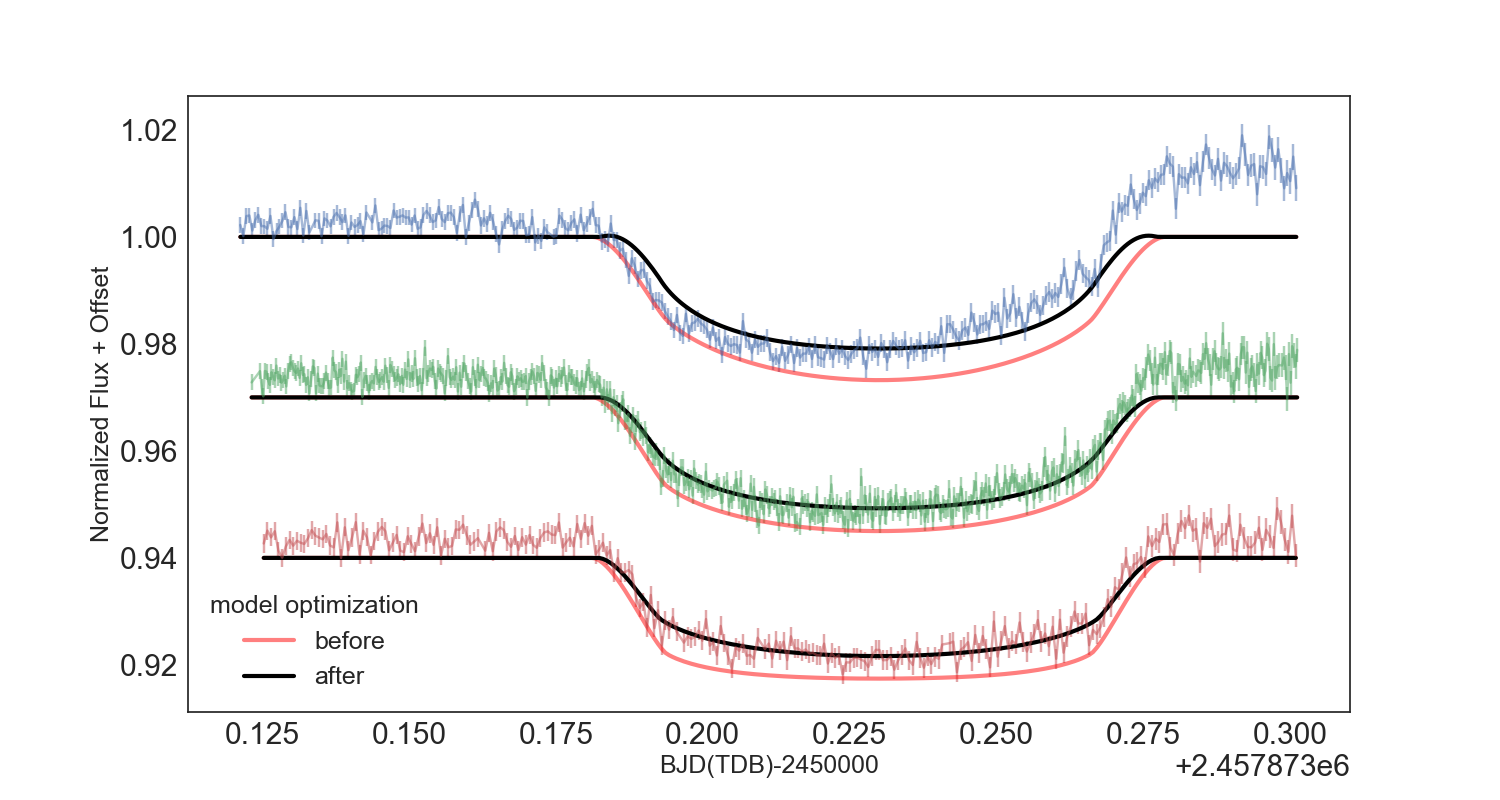
\includegraphics[width=12cm]{hatp44/optimized_transit_model.png}
\caption{Comparison of transit model before (red solid line) and after (black) optimization. As usual, the blue, green, and red light data points with error bars correspond to g-,r-, and z-bands, respectively. The light curves as displaced vertically for clarity.}
\label{fig:hatp44_opt}
\end{figure}

\begin{figure}
\centering
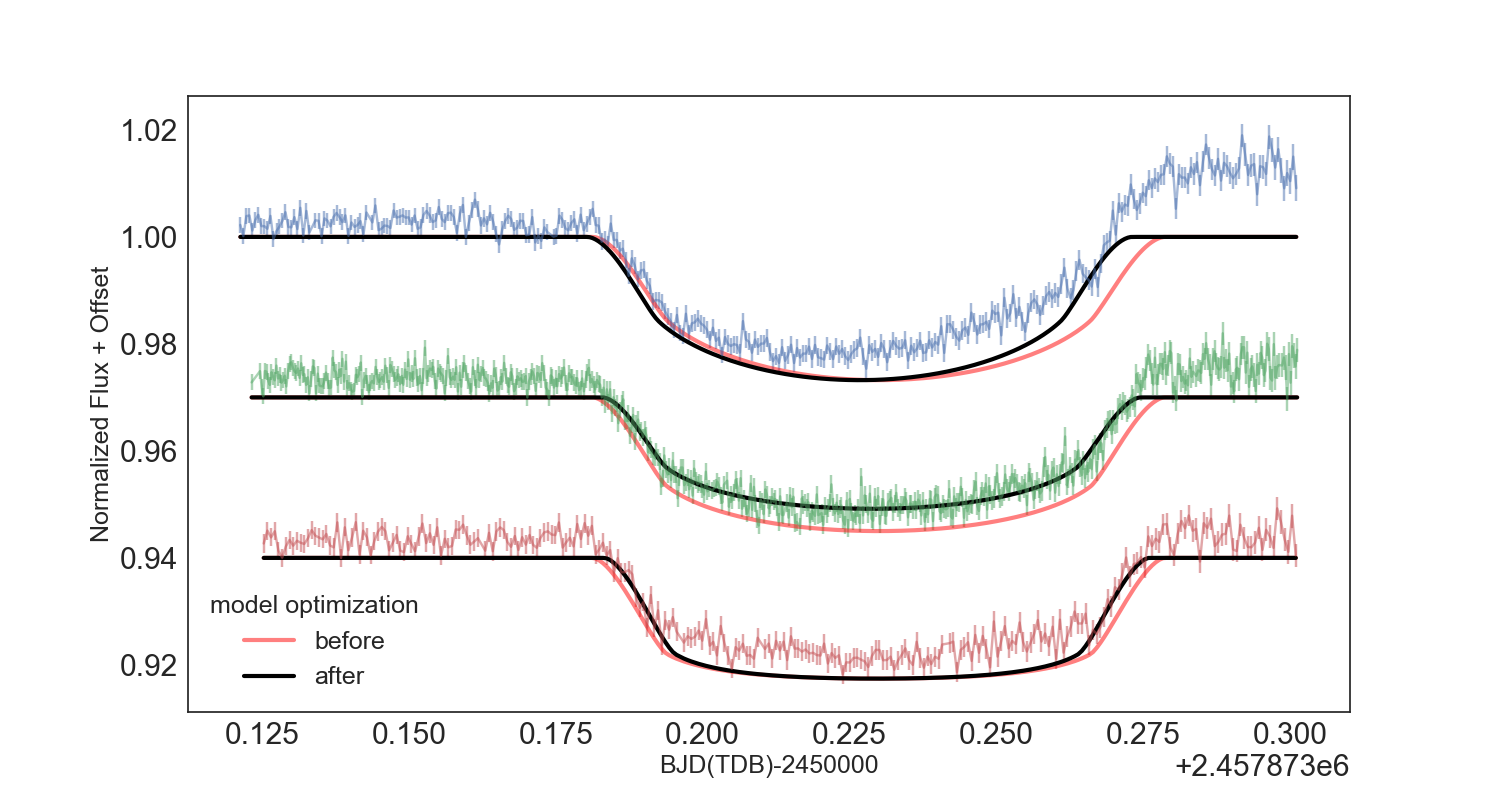
\includegraphics[width=12cm]{hatp12/optimized_transit_model.png}
\caption{Same as Fig.~\ref{fig:hatp44_opt} but for HAT-P-12b.}
\label{fig:hatp12_opt}
\end{figure}

\begin{figure}
\centering
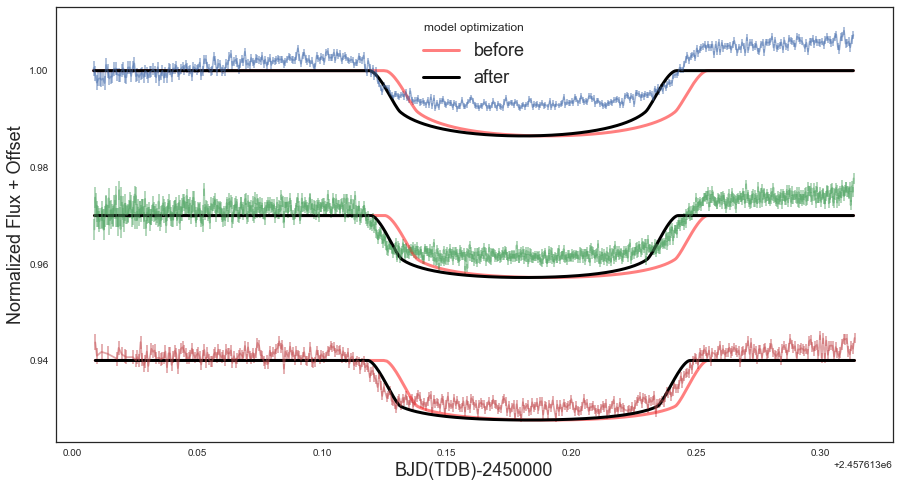
\includegraphics[width=12cm]{wasp21/optimized_transit_model.png}
\caption{Same as Fig.~\ref{fig:hatp44_opt} but for WASP-21b}
\label{fig:wasp21_opt}
\end{figure}

%reduced chi-square
After optimization, we re-scale the photometric errors to take into account possible over-/under-fitting and red noise in the residual. First, we inflate the original estimate of the photometric uncertainty such that the reduced $\chi^2$ for each light curve becomes unity. Reduced $\chi^2$ is defined as
\begin{equation}
red. \chi^2= \frac{\chi^2}{n-d}
\end{equation}
where $n$ is the number of data points and $d$ is the number of parameters.

%beta: time-correlated noise
Second, we estimate the level of time-correlated noise (a.k.a. red noise: Pont et al. 2006) in each light curve, by calculating the $\beta$ factor at various bins (Winn et al. 2008). 
%The $\beta$ factor is used to take into account the time-correlated noise and to properly compensate for the possible underestimation of derived uncertainties from our analysis . 
Specifically, the beta factor is defined as
\begin{equation} \label{eq:beta}
\sigma_N = \frac{\sigma_1}{\sqrt{N}}\sqrt{\frac{M}{M-1}}
\end{equation}
where $\sigma_n$ is the theoretical standard deviation of the binned residuals, $\sigma_1$ is the standard deviation of the unbinned residuals, $N$ is the number of data points per bin, and $M$ is the number of bins. We then compute the median value of $\beta$ for all values of $N$ corresponding to bin widths between 5-20-minute as illustrated in Fig.~\ref{fig:beta} for the case of HAT-P-44b.
%The light curves show significant time-correlated noise, especially in the r- and z-band. 
If the reduced $\chi^2$ and/or $\beta$ is larger than unity, we re-scale the photometric errors of the data; else we preserve the original estimate of the uncertainty to be conservative. The computed $\chi^2$ and $\beta$ values for various binning cases in each color are summarized in Table~\ref{tab:beta}.
Fig.~\ref{fig:rms} shows a similar diagnosis for red noise which compares the rms of the residual as a function of bin size with the theoretical $\sqrt{n}$ decrease expected for Poisson noise.


\begin{figure}
\centering
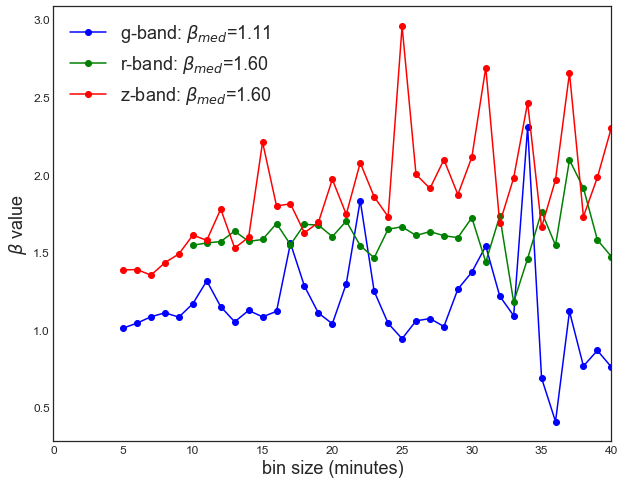
\includegraphics[width=8cm]{figures/beta.png}
\caption{Beta values computed at different binning for HAT-P-44b in each band as a measure of time-correlated (a.k.a. red) noise in the light curve. The median values of betas at all bin-sizes indicated in the upper left are used to inflate the original photometric uncertainties.}
\label{fig:beta}
\end{figure}

\begin{figure}
\centering
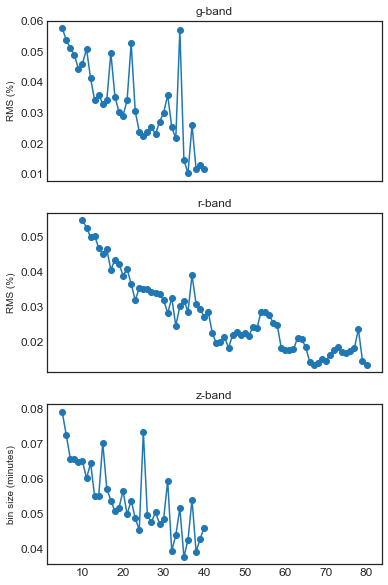
\includegraphics[width=8cm]{figures/binned_rms.png}
\caption{Computed rms error of the residual as function of bin sizes in each color of HAT-P-44b light curve. The monotonic ($\sqrt{n}$) decrease in rms as function of bin size is expected for residual which is purely Poisson noise.}
\label{fig:rms}
\end{figure}

\begin{table}
\centering
\caption{Computed reduced chi-square and beta values used to re-scale the original estimate of photometric uncertainty.}
\label{tab:beta}
\begin{tabular}{llllll}
\multicolumn{2}{l}{}                    & HAT-P-44  & HAT-P-12 & WASP-21 \\ \hline
\multirow{3}{*}{red. $\chi^2$} & g-band: & 1.0963   & 1.4076  & 2.8091\\
                              & r-band: & 1.0971    & 1.6511  & 2.0338\\
                              & z-band: & 1.0487    & 1.2946  & 1.7551\\ \hline
$\beta$                       & g-band: & 1.1515 & 2.5096     & 3.3068 \\
                              & r-band: & 1.3033 & 4.2240     & 4.6869 \\
                              & z-band: & 1.3345 & 1.8684     & 2.9127 \\  \hline
\end{tabular}
\end{table}

\subsection{Markov Chain Monte Carlo \label{sec:MCMC}}
%We derived the maximum posterior probability distributions for the fitted parameters by solving the Bayesian relation and running multiple, very long Monte Carlo Markov Chain (MCMC) simulations of our multivariate model. 
Markov Chain Monte Carlo (MCMC) methods are a class algorithms used to sample from--and thereby provide sampling approximations to--the posterior probability distribution function (PDF) efficiently even in parameter spaces with high number of dimensions. Detailed discussion of MCMC is beyond the scope of this thesis and so only the relevant information is summarized as follows.

The goal of our MCMC simulation is to generate a chain of states, i.e. a chain of sets of model parameters $\theta_i$ that are sampled from the desired posterior PDF $P(\theta|D)$. Using the simple Metropolis-Hastings algorithm for example, such a chain can be computed by specifying an initial set of parameter values, $\theta_0$, and a proposal distribution, $P(\theta$'|$\theta_n)$. At each iteration, a new proposal state $\theta$' is generated and the corresponding model is fit to the data. The new proposal state is then randomly accepted or rejected with a probability that depends on (1) difference between the $\chi^2$-fits of the previous state and the proposal state and (2) difference in the prior probability between previous state and prior state. A proposal state that leads to an improvement in the $\chi^2$-fit and a higher prior probability compared to the previous state is always accepted. The process is repeated long enough until the chains are sufficiently converged. From the posterior PDF, several statistical measures can be computed including the best estimates and Bayesian credible regions. On this note, the prior uncertainties associated with the free parameters are propagated to the final estimate.

Note that MCMC is a necessary step in our transit modeling because the result of the non-linear optimization in \S \ref{sec:optimization} may not necessarily correspond to the global optimum solution. Especially in the case of our modeling which requires exploring large dimensional hyper-surface (>20 free parameters), MCMC is a robust method to obtain such a solution.

\paragraph{MCMC Set-up}
%In the per color set-up, all transit (except period) and systematics model parameters are kept free. 
Instead of modeling light curves individually, we modeled all light curves (g-,r-, and z-bands) simultaneously. The advantage of simultaneous multi-color modeling is leveraging mutual information in each color such as $t_c, b$, and $a_s$ at the expense of having higher total number of parameters. In this set-up, we fitted the three light curves simultaneously by treating $R_p/R_s$ and $q_1, q_2$, and $w$ as independent free parameters for each band while treating $t_c, b$, and $a_s$ as common/ shared (i.e. color-independent) parameter. Except for the period, %passband-dependent
transit parameters and systematics coefficients listed in Table \ref{tab:param_mcmc} are kept free. %As a consistency check, we compare the result of per color modeling and confirm both give consistent results.

\begin{table}
\centering
\caption{Parameter setting matrix for our MCMC run}
\label{tab:param_mcmc}
\begin{tabular}{llllll}
                     & Fixed   & Free   \\ \hline
Shared      & $P$     & $t_c, b, a_s$   \\
Independent &         & $q_{1,i},q_{2,i}, k_i, w_i$ \\
\hline
\end{tabular} \\
\raggedright \textbf{Notes.} The parameters assigned with subscript $i$, are color-dependent. In per color set-up, there are 6 transit parameters and 5 coefficients $w_i$, amounting to 11 free parameters. In the multi-color set-up, $b$, $a_s$, and $t_c$ are shared amounting to 27 free parameters in the MCMC run. 
\end{table}

We use \verb'emcee'\footnote{http://github.com/dfm/emcee}, an affine-invariant ensemble sampler (\cite{Foreman-Mackey2013}) with 256 walkers which ran for 10$^5$ steps starting from the optimized values computed in $\S$\ref{sec:optimization} taken as initial values. 
After discarding the first 10\% steps (i.e. burn-in phase),  
%Gelman-Rubin statistic
we combined the results from all chains and evaluated convergence of each parameter using the Gelman-Rubin statistic $\hat{R}$ (Gelman \& Rubin 1992), and considered the chains to be stabilized %well-mixed 
if $\hat{R} \leq 1.05$ for all parameters. To ensure independent sampling, we constructed the posterior distribution by sampling each chain at intervals spaced by autocorrelation time scale, $\tau$.  %The autocorrelation time is a direct measure of the number of evaluations of the posterior PDF required to produce independent samples of the target density.
%The full set of maximum aposteriori (MAP) values based on the highest log probability should converge to/consistent within one sigma with the individual median values.
% The jump sizes of parameters in each MCMC step are adjusted such that acceptance ratios become ∼23%, which is considered as an optimal acceptance ratio for efficient convergence of MCMC (see e.g., Ford 2005).
We tested for convergence by dividing the chain in two halves and confirmed that they gave consistent results. We also took 10$^3$ independent samples in each chain and plotted the results as shown in Fig.~\ref{fig:hatp44_samples}--\ref{fig:wasp21_samples}.
%The mean values of the parameter traces were then interpreted as the most probable parameters utilizing the 68.3\% highest probability density intervals (HPD) as our error estimate. %For those parameters which require error propagation, such as the impact parameter $b$, we applied the corresponding equation to the MCMC parameter traces; then the HPD of the parameter can be determined from that new distribution.
We checked that maximum posterior probability distributions of wavelength-independent parameters such as scaled semi-major axis, $a/R_s$, impact parameter, $b$, and transit center, $t_c$, 
%stellar density, $\rho_s$ 
are consistent within 1-$\sigma$ in both set-ups. %as shown in Table~\ref{tab:MAP}. 
We define 1$\sigma$ uncertainties by the range of parameters between 15.87\% and 84.13\% of the merged posterior distributions. The results are described in $\S$ \ref{sec:results}. 